\documentclass[border=8pt]{standalone}
\usepackage{tikz}
\usetikzlibrary{arrows.meta, positioning, calc, fit, backgrounds, decorations.pathreplacing}
\usepackage{amsmath, amssymb, amsfonts}
\usepackage{xcolor}

% Custom math commands (mirror main.tex preamble)
\newcommand{\loss}{\mathcal{L}}
\newcommand{\encoder}{f}
\newcommand{\probe}{h}

\definecolor{audblue}{RGB}{70,110,180}
\definecolor{visora}{RGB}{220,135,55}
\definecolor{probegr}{RGB}{60,135,75}

\begin{document}
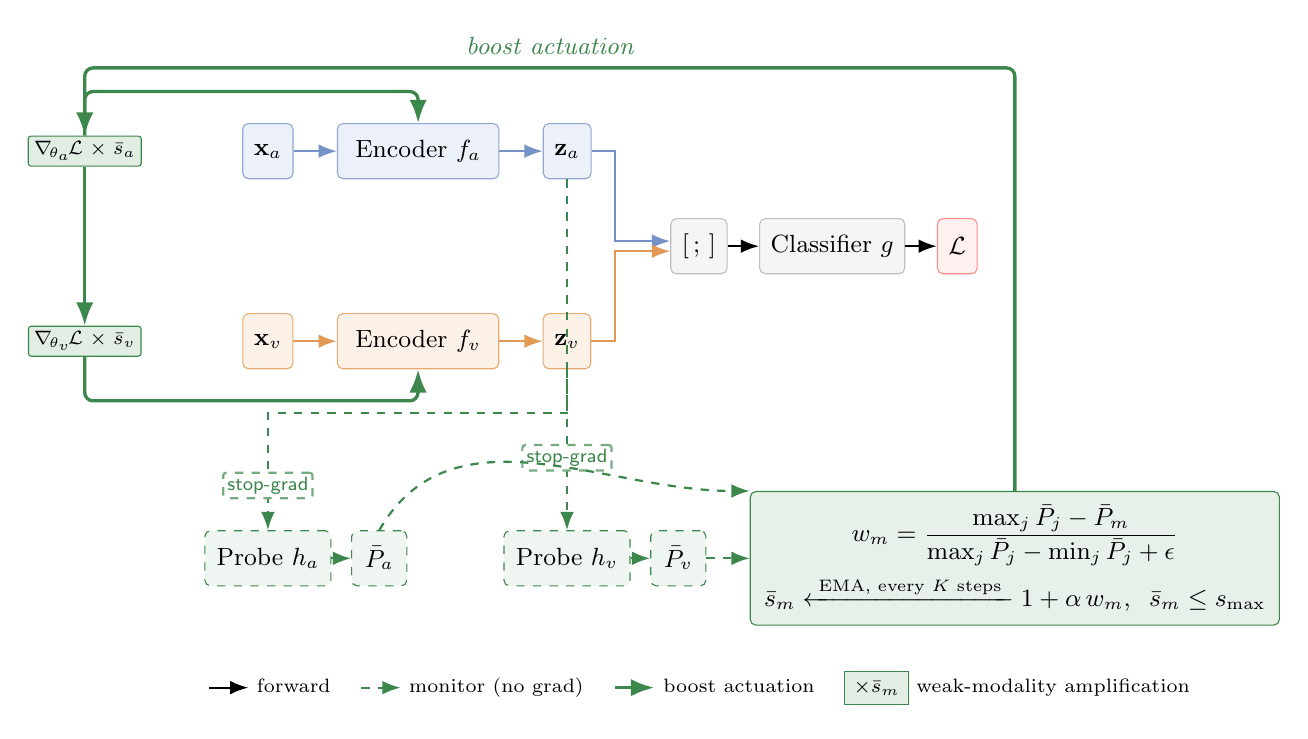
\begin{tikzpicture}[
    >=Latex,
    box/.style={draw, rounded corners=2pt, minimum height=0.7cm,
                font=\small, align=center, inner sep=4pt},
    arr/.style={->, thick},
    farr/.style={->, thick},
    darr/.style={->, thick, dashed, probegr},
    barr/.style={->, very thick, probegr},
    btag/.style={fill=probegr!15, draw=probegr, rounded corners=1pt,
                 font=\scriptsize, inner sep=2pt, text=black},
    sgbadge/.style={fill=white, draw=probegr!70, rounded corners=1pt,
                    font=\scriptsize\sffamily, inner sep=1.5pt},
]

\node[box, fill=audblue!10, draw=audblue!60] (xa) {$\mathbf{x}_a$};
\node[box, fill=audblue!10, draw=audblue!60, right=0.55cm of xa, minimum width=2.05cm] (fa)
    {Encoder $\encoder_a$};
\node[box, fill=audblue!10, draw=audblue!60, right=0.55cm of fa] (za) {$\mathbf{z}_a$};

\node[box, fill=visora!12, draw=visora!70, below=1.7cm of xa] (xv) {$\mathbf{x}_v$};
\node[box, fill=visora!12, draw=visora!70, right=0.55cm of xv, minimum width=2.05cm] (fv)
    {Encoder $\encoder_v$};
\node[box, fill=visora!12, draw=visora!70, right=0.55cm of fv] (zv) {$\mathbf{z}_v$};

\node[box, fill=gray!8, draw=gray!50,
      right=1.0cm of $(za.east)!0.5!(zv.east)$] (concat) {$[\,;\,]$};
\node[box, fill=gray!8, draw=gray!50, right=0.4cm of concat, minimum width=1.7cm] (g)
    {Classifier $g$};
\node[box, fill=red!6, draw=red!45, right=0.4cm of g] (loss) {$\loss$};

\draw[farr, audblue!75] (xa) -- (fa);
\draw[farr, audblue!75] (fa) -- (za);
\draw[farr, visora!85] (xv) -- (fv);
\draw[farr, visora!85] (fv) -- (zv);
\draw[farr, audblue!75] (za.east) -- ++(0.3,0) |- (concat.170);
\draw[farr, visora!85] (zv.east) -- ++(0.3,0) |- (concat.190);
\draw[farr] (concat) -- (g);
\draw[farr] (g) -- (loss);

\coordinate (boostCol) at ([xshift=-2.0cm]xa.west);
\node[btag, anchor=center] at (boostCol |- fa) (bfa)
    {$\nabla_{\!\theta_a}\!\loss\;{\times}\;\bar{s}_a$};
\node[btag, anchor=center] at (boostCol |- fv) (bfv)
    {$\nabla_{\!\theta_v}\!\loss\;{\times}\;\bar{s}_v$};

\draw[barr, rounded corners=3pt]
    (bfa.north) |- ([yshift=0.4cm]fa.north) -- (fa.north);
\draw[barr, rounded corners=3pt]
    (bfv.south) |- ([yshift=-0.4cm]fv.south) -- (fv.south);

\coordinate (probeRow) at ([yshift=-2.4cm]fv.south);

\node[box, fill=probegr!8, draw=probegr, dashed, minimum width=1.6cm]
    at (probeRow -| xv) (pa) {Probe $\probe_a$};
\node[box, fill=probegr!8, draw=probegr, dashed,
      right=0.25cm of pa, inner sep=3pt, minimum width=0.7cm] (Pa) {$\bar{P}_a$};
\node[box, fill=probegr!8, draw=probegr, dashed, minimum width=1.6cm]
    at (probeRow -| zv) (pv) {Probe $\probe_v$};
\node[box, fill=probegr!8, draw=probegr, dashed,
      right=0.25cm of pv, inner sep=3pt, minimum width=0.7cm] (Pv) {$\bar{P}_v$};

\node[box, fill=probegr!12, draw=probegr, align=center,
      right=0.55cm of Pv, inner sep=5pt, minimum width=4.4cm] (boost)
    {$w_m = \dfrac{\max_j \bar{P}_j - \bar{P}_m}{\max_j \bar{P}_j - \min_j \bar{P}_j + \epsilon}$\\[3pt]
     $\bar{s}_m \xleftarrow{\;\text{EMA, every } K \text{ steps}\;} 1 + \alpha\, w_m,\;\;\bar{s}_m \le s_{\max}$};

\draw[darr]
    (za.south) -- ([yshift=-0.55cm]fv.south -| za)
              -- ([yshift=-0.55cm]fv.south -| pa)
              -- (pa.north)
    node[sgbadge, pos=0.62] {stop-grad};
\draw[darr] (zv.south) -- (pv.north)
    node[sgbadge, pos=0.55] {stop-grad};

\draw[darr] (pa.east) -- (Pa.west);
\draw[darr] (pv.east) -- (Pv.west);

\draw[darr] (Pv.east) -- (boost.west);
\draw[darr] (Pa.north) to[out=60,in=180] (boost.north west);

\coordinate (railTopY) at ([yshift=0.7cm]fa.north);
\coordinate (railR) at (boost.north |- railTopY);
\coordinate (railL) at (bfa.north |- railTopY);

\draw[barr, rounded corners=3pt]
    (boost.north) -- (boost.north |- railTopY)
                  -- (railL)
                  -- (bfa.north);

\draw[barr] (bfa.south) -- (bfv.north);

\node[font=\small\itshape, probegr, anchor=south]
    at ([yshift=0.05cm]$(railL)!0.5!(railR)$) {boost actuation};

\coordinate (legendAnchor) at ([yshift=-1.0cm]pa.south -| concat);
\node[anchor=north, font=\scriptsize, inner sep=2pt] at (legendAnchor) {%
  \tikz[baseline=-0.6ex]\draw[->,thick] (0,0)--(0.5,0);~forward \quad
  \tikz[baseline=-0.6ex]\draw[->,thick,dashed,probegr] (0,0)--(0.5,0);~monitor (no grad) \quad
  \tikz[baseline=-0.6ex]\draw[->,very thick,probegr] (0,0)--(0.5,0);~boost actuation \quad
  \fcolorbox{probegr}{probegr!15}{\scriptsize$\times\bar{s}_m$}~weak-modality amplification
};

\end{tikzpicture}
\end{document}
